\section{Appendix}



\subsection{Part 1}
\subsubsection{SVM illustration}
\label{appendix:part1svm}
\begin{figure*}[ht]
	\centering 
	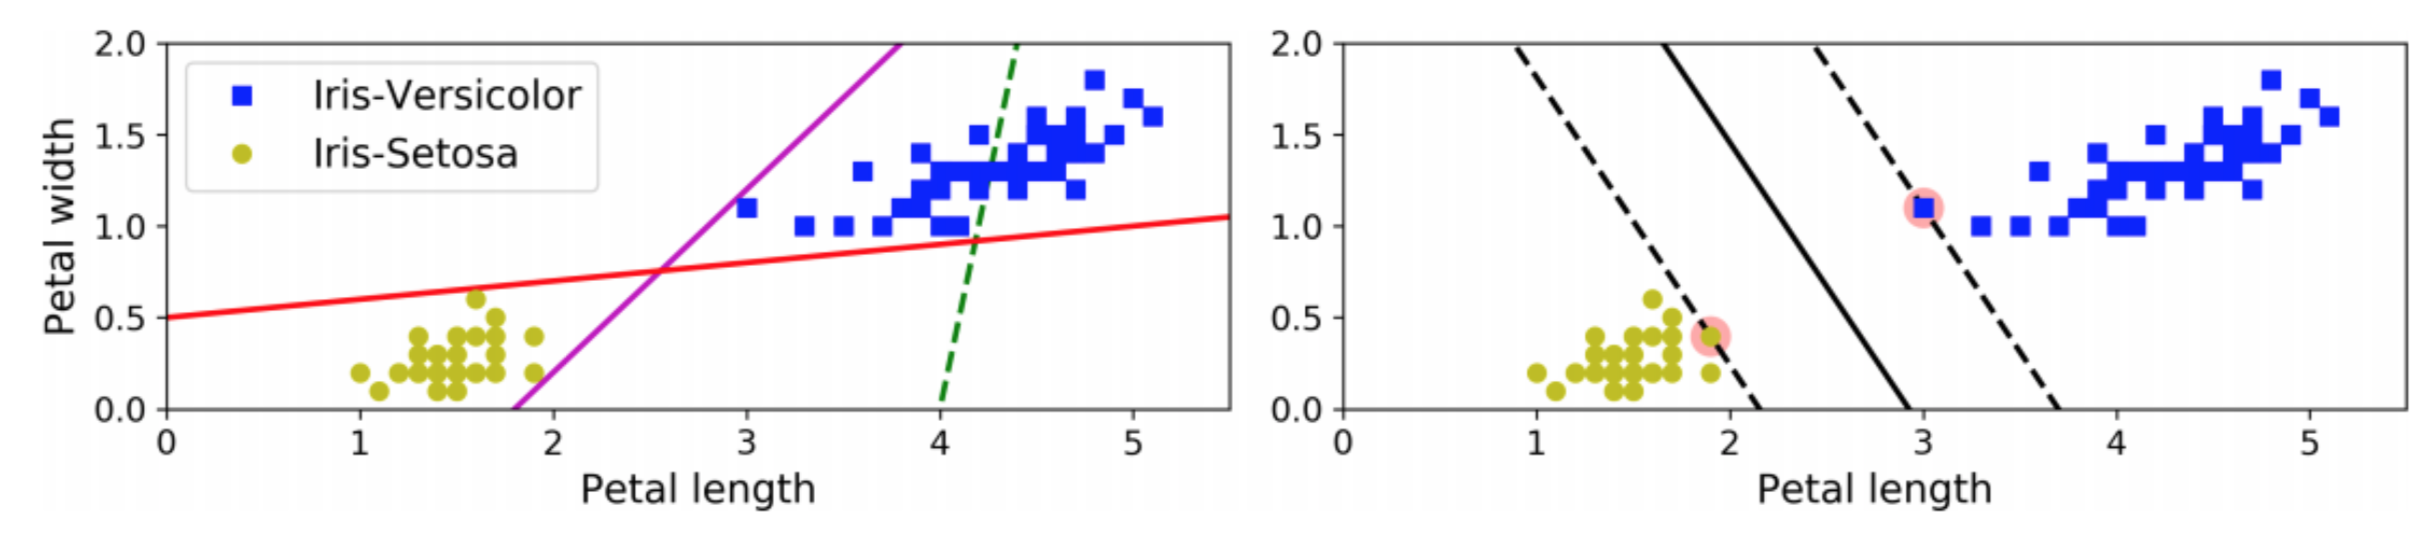
\includegraphics[scale = 0.3]{Pics/SVM}
	\caption{SVM illustration}
	\label{fig:svmex}
\end{figure*}

On this figure we see two plots representing one same problem of separation. The one on the left is drawing several linear separations possible. The red and purple ones would correctly separate the data. But the purpose of the SVM is to maximise the margins around the boundary. That is why the optimised boundary is the one on the right as it maximises the distance between the closest data point and the linear boundary. 

\subsubsection{Changing the loss function : confusion matrix / heatmap}
\label{appendix:changingloss}
\begin{figure*}[h]
	\centering 
	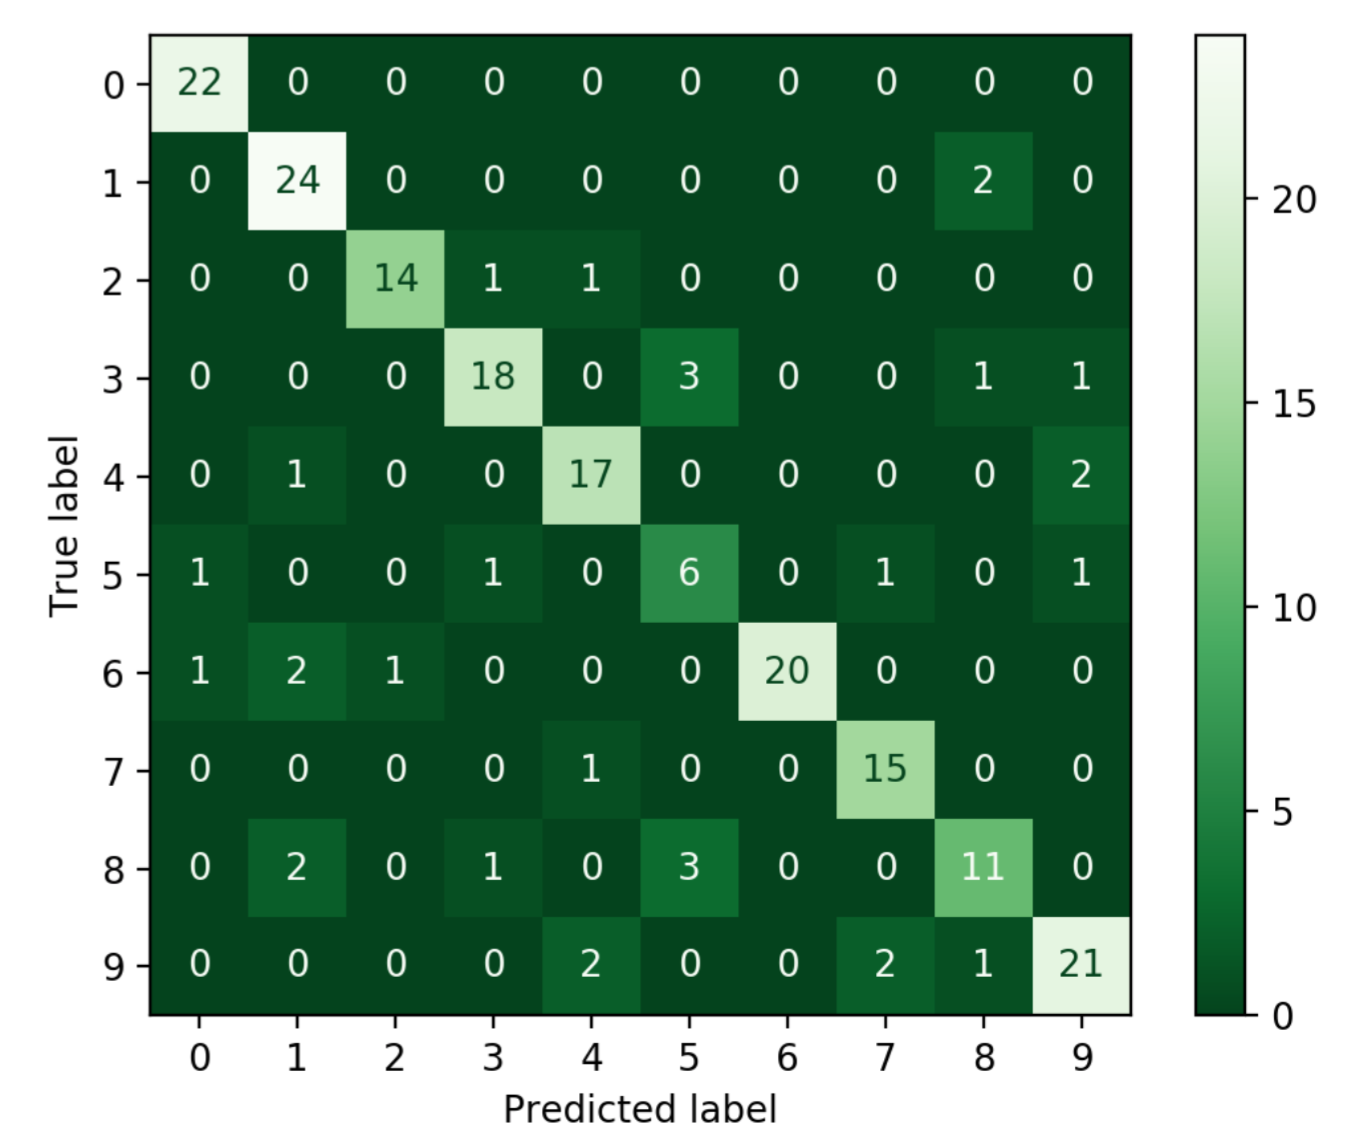
\includegraphics[scale=0.4]{Pics/confusion_matrixr}
	\caption{Confusion matrix for the SVM classifier}
	\label{fig:confusion}
\end{figure*}

\newpage

\subsection{Part 2}
\subsubsection{Algorithm}
\label{appendix:algo}
\begin{figure*}[h]
	\centering 
	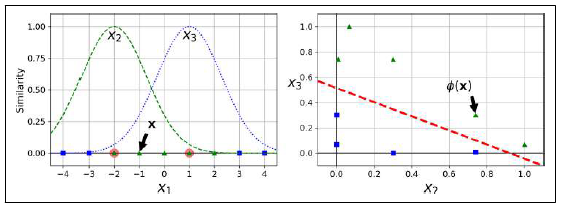
\includegraphics{Pics/RBF}
	\caption{Similarity features using the Gaussian RBF}
	\label{fig:rbfgaussian}
\end{figure*} 

\subsubsection{Final confusion matrix}
\begin{figure*}[h]
	\centering 
	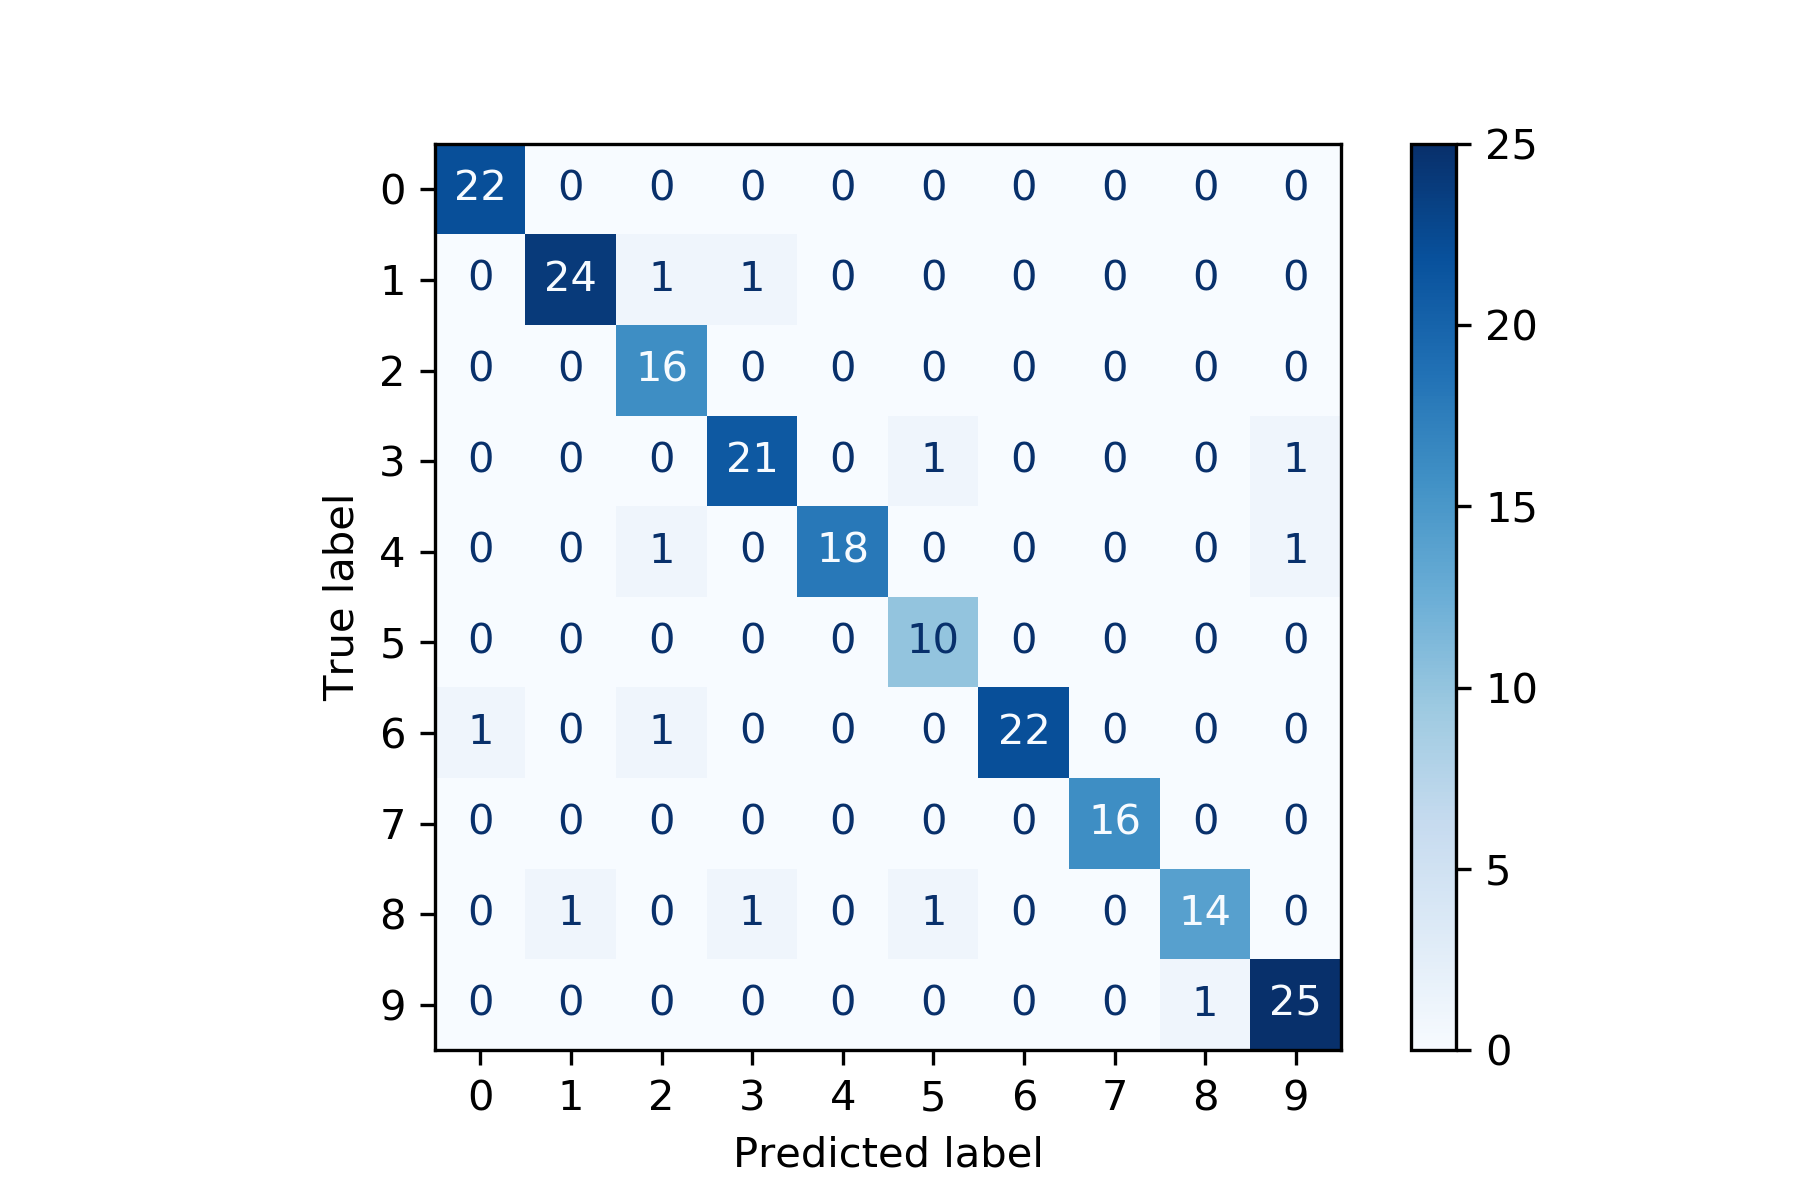
\includegraphics[scale=0.9]{Pics/part2confusion_mat}
	\caption{Confusion matrix part 2}
	\label{fig:confusion}
\end{figure*} 

